\section{Numerical operator and implementation}
\label{app:appendix_math}

\subsection{Finite Newton--Schulz map}

The executed map uses ten polynomial iterations in mixed precision, so it is not an exact SVD polar factor. For $Z=LUR$, we first compute $X_0=Z/(\|Z\|_F+10^{-5})$ in FP32. Tall matrices are transposed so each Gram has dimension $\min(m,n)$. For $k=0,\ldots,9$,
\begin{equation}
 A_k=X_k\star X_k^{\Tr},\qquad
 X_{k+1}=3.4445X_k+[-4.7750A_k+2.0315(A_k\star A_k)]\star X_k,
 \label{eq:ns10}
\end{equation}
where $P\star Q$ rounds both operands to BF16 and accumulates the matrix product in FP32. Scalar combinations stay in FP32, and tall results are transposed back. The exact identity in \Cref{eq:som_rotation} is a reference for understanding this operator, not an exact description of every finite-iteration update.

The recorded sensitivity check perturbs each FP32 input element by one ULP. The perturbation grows through iterations 3--10 to a $5.2\times10^{-4}$ parameter-delta shift under this rounding path; perturbing outer factors gives a $1.9\times10^{-9}$ shift. These checks motivate the unified execution path and \mname{Null-WT} comparison. Deterministic runs use \texttt{CUBLAS\_WORKSPACE\_CONFIG=:4096:8}.

\subsection{Dense products and cotangent capture}

Dense products outside the Newton--Schulz map use an FP16-split Tensor-Core implementation. With TF32 disabled, this avoids the slow native FP32 path on A100. For a tensor $X$, the split uses $s=2^{13-\lfloor\log_2\max|X|\rfloor}$, $X_{\rm hi}=\operatorname{half}(sX)$, and $X_{\rm lo}=\operatorname{half}(4096(sX-\operatorname{float}(X_{\rm hi})))$. The recorded product audit finds relative error below $3\times10^{-7}$ against FP64 references. This is an empirical arithmetic check for the tested matrices.

Backward capture receives loss-scaled cotangents. For $G_{\rm acc}$ microbatches, $B_{\rm micro}$ sequences, and 4,095 scored targets per sequence, autograd returns the summed-loss derivative divided by $B_{\rm micro}\,4095\,G_{\rm acc}$. Capture applies a fixed $2^{16}$ scale before BF16 storage and FP32 accumulation to reduce underflow. Raw sums and sample counts are pooled across ranks before the EMA update. Trace normalization cancels a common constant scale in exact arithmetic; finite-precision capture can still introduce rounding error.

\subsection{Metric-shaped weight decay and control scope}
\label{app:weight_decay}

Writing the decoupled matrix update in \cref{eq:update} as $W_{p,t+1}=W_{p,t}-\eta_t(s_{m_p,n_p}D_{p,t}+\lambda Q_{p,t})$ separates the preconditioned descent direction $D_{p,t}$ from the weight-decay operator $Q_{p,t}$. In \mname{MuonT}, \mname{OD-All}, \mname{WT-MLP}, and \mname{WT-MLP-Lag}, we set $Q_{p,t}=W_{p,t}\hat R_{p,t}^2$. This right-shaped decay rule is inherited from \mname{MuonT}~\citep{mohamadi2026toner} and arises from applying isotropic $\ell_2$ weight decay in the right-reparameterized coordinates $W=\widetilde W\hat R$, with $\hat R=\unitrms(A_n(C)^{-1/8})\succ0$ held fixed at step $t$. Expressing $\mathcal R(W)=\frac{\lambda}{2}\|W\|_F^2=\frac{\lambda}{2}\|\widetilde W\hat R\|_F^2$ in $\widetilde W$-coordinates gives gradient $\nabla_{\widetilde W}\mathcal R=(\nabla_W\mathcal R)\hat R^{\Tr}=\lambda W\hat R$. Taking a decoupled step $\Delta\widetilde W_{\rm wd}=-\eta_t\lambda W\hat R$ and mapping back to $W$-space via $\Delta W_{\rm wd}=(\Delta\widetilde W_{\rm wd})\hat R$ multiplies on the right by $\hat R$ a second time:
\[
 \Delta W_{\rm wd}=-\eta_t\lambda(W\hat R)\hat R=-\eta_t\lambda W\hat R^2,
\]
which equals the Euclidean gradient step on $\frac{\lambda}{2}\|W\hat R\|_F^2=\frac{\lambda}{2}\tr(W\hat R^2 W^{\Tr})$ with respect to $W$ at fixed $\hat R$. Because $\hat R$ has unit RMS, $\frac{1}{n}\|\hat R\|_F^2=\frac{1}{n}\tr(\hat R^2)=1$, so $\hat R^2$ has unit mean eigenvalue: overall decay strength remains $\lambda$ while relative shrinkage across input eigendirections matches the post-polar right scaling $\hat R$ in $D_{p,t}$.

Holding $Q=W\hat R^2$ fixed across \mname{MuonT}, \mname{OD-All}, \mname{WT-MLP}, and \mname{WT-MLP-Lag} ensures that our main scaling and ablation comparisons (\Cref{sec:scaling,sec:controls_ablations}) isolate the output-preconditioned direction $D_{p,t}$ without simultaneously changing the regularizer. Conversely, the two-sided polar baseline comparison in \Cref{sec:related_baselines} (\Cref{tab:related}) evaluates \mname{Muon}, \mname{GO-MUON}, \mname{Mousse}, and synchronous \mname{WT-MLP} under shared isotropic decay $Q=W$, verifying that width-thresholded output preconditioning retains its held-out gain without right-shaped decay. In our exploratory placement ledger (\Cref{sec:ablations,tab:ablations_full}), output-only replacement (\mname{Abl-OutOnly}, where $R=\hat R=I$) uses $Q=\hat L^2 W$ whereas \mname{Muon} uses $Q=W$, so \mname{Abl-OutOnly} alters both $D_{p,t}$ and $Q_{p,t}$ and cannot alone isolate input whitening.

\subsection{Why output preconditioning omits left-shaped weight decay}
\label{app:left_decay_asymmetry}

\paragraph{Inner polar rotation versus outer post-polar scaling.}
In \mname{WT-MLP-Lag}, output preconditioning enters through two distinct factors around the polar map: the pre-polar inner root $L=A_m(B)^{-1/2}$ inside $\Nten(LUR)$ (or $L^{\mathsf{Diag}}$ at width $\dff$) and the post-polar outer root $\hat L=\unitrms(A_m(B)^{-1/8})$ (or $\hat L^{\mathsf{Diag}}$). Under the exact row-polar identity \cref{eq:som_rotation} (\Cref{sec:mechanism}), left-multiplying a full-row-rank matrix ($m\le n$, covering \texttt{q,k,v,o,down}) by symmetric positive-definite $L$ inside the polar factor acts purely as an orthogonal left rotation $\Omega\in SO(m)$ on row space. Because the Frobenius penalty $\mathcal R(W)=\frac{\lambda}{2}\|W\|_F^2$ is orthogonally invariant ($\|\Omega^{\Tr}W\|_F^2=\|W\|_F^2$), an orthogonal row reparameterization $W=\Omega\widetilde W$ gives $\nabla_{\widetilde W}\mathcal R=\lambda\Omega^{\Tr}W$ and maps back to $\Delta W_{\rm wd}=-\eta_t\lambda\Omega\Omega^{\Tr}W=-\eta_t\lambda W$: pure left-side polar rotation leaves Euclidean weight decay identically unchanged (likewise, for tall full-column-rank matrices with $m>n$, inner left multiplication reorients the semi-orthogonal Stiefel frame without scaling singular values). By contrast, extending the linear reparameterization to include post-polar symmetric scaling on both sides, $W=\hat L\widetilde W\hat R$ with $\hat L,\hat R\succ0$ held fixed at step $t$, transforms $\mathcal R(W)=\frac{\lambda}{2}\|\hat L\widetilde W\hat R\|_F^2$ into gradient $\nabla_{\widetilde W}\mathcal R=\lambda\hat L W\hat R$. Taking a decoupled step $\Delta\widetilde W_{\rm wd}=-\eta_t\lambda\hat L W\hat R$ and mapping back via $\Delta W_{\rm wd}=\hat L(\Delta\widetilde W_{\rm wd})\hat R$ yields the symmetric two-sided decay operator
\[
 \Delta W_{\rm wd}^{\rm sym}=-\eta_t\lambda\hat L^2 W\hat R^2,
\]
which is the Euclidean gradient step on $\frac{\lambda}{2}\|\hat L W\hat R\|_F^2=\frac{\lambda}{2}\tr(\hat L^2 W\hat R^2 W^{\Tr})$ with respect to $W$ at fixed $(\hat L,\hat R)$. Any left-side metric shaping of weight decay is therefore induced solely by the post-polar outer factor $\hat L$.

\paragraph{Dynamical asymmetry between input and output shaping.}
Despite the formal duality between activations and cotangents in $G=\sum_j\delta_j x_j^{\Tr}$, left-multiplying weight decay by $\hat L^2$ behaves asymmetrically from right-multiplying by $\hat R^2$ for a linear projection $y=Wx$ because $W$ does not generate its own input $x$, whereas $W$ directly generates its own output $y$:
\begin{enumerate}
 \item \emph{Inverse-power feedback along quiet output channels.} Because $\hat L^2\propto A_m(B)^{-1/4}=(\tilde B+\epsilon I_m)^{-1/4}$ (and $(\hat L^{\mathsf{Diag}})^2\propto\Diag(a^{-1/4})$ with $a_i=\tilde B_{ii}+\epsilon$ in \cref{eq:diag_roots}) carries a negative exponent of the cotangent second moment, output directions with smaller cotangent variance receive larger decay multipliers $\hat L^2$, while unit-RMS normalization ($\frac{1}{m}\tr(\hat L^2)=1$) correspondingly relaxes weight decay ($\hat L^2<1$) along high-variance, oscillatory cotangent modes. On the input side, shrinking a column of $W$ does not attenuate upstream RMSNormed activations $x$. On the output side—most transparently in gated MLP projections $z=\operatorname{SiLU}(W_{\rm gate}x)\odot(W_{\rm up}x)$ with upstream cotangent $g_z=\partial\ell/\partial z$, where $\delta_{{\rm gate},i}=g_{z,i}\operatorname{SiLU}'(y_{{\rm gate},i})\,y_{{\rm up},i}$ and $\delta_{{\rm up},i}=g_{z,i}\operatorname{SiLU}(y_{{\rm gate},i})$—a small row norm in one branch reduces its forward activation magnitude ($y_{{\rm up},i}$ or $\operatorname{SiLU}(y_{{\rm gate},i})$), multiplicatively attenuating backpropagated cotangents into the sibling branch, lowering $B_{ii}$, and increasing $\hat L_{ii}^2\propto a_i^{-1/4}$. Left-shaped decay thus risks positive-feedback shrinkage on quiet output units alongside weakened regularization on volatile cotangent modes.
 \item \emph{Non-stationary regularization metric and dense product cost.} As measured in \Cref{sec:drift_cost} (\Cref{tab:diagnosis_summary}), RMSNormed input eigenspaces evolve slowly ($\mathrm{Drift}_{16}\approx 0.021$ over 250 steps), so $W\hat R^2$ acts as a nearly stationary quadratic regularizer across many updates. Output cotangent eigenspaces rotate roughly an order of magnitude faster ($\mathrm{Drift}_{16}\approx 0.11\text{--}0.66$), so $\hat L_{t-1}^2 W\hat R^2$ subjects weights to a rapidly rotating penalty ellipsoid $\frac{\lambda}{2}\tr(\hat L_{t-1}^2 W\hat R^2 W^{\Tr})$ while requiring an extra dense $\dm\times\dm$ left matrix product per step on each of the five hidden-width projections (\texttt{q,k,v,o,down}).
\end{enumerate}

\paragraph{Epistemic scope.}
These two dynamical mechanisms serve as structural motivations—alongside experimental isolation relative to \mname{MuonT} (\Cref{app:weight_decay})—for retaining one-sided $Q=W\hat R^2$ in \mname{WT-MLP-Lag}, rather than an empirical proof that $Q=\hat L_{t-\tau}^2 W\hat R^2$ degrades or destabilizes training. Evaluating $Q\in\{W, W\hat R^2, \hat L_{t-\tau}^2 W\hat R^2\}$ while holding the preconditioned descent direction $D_{p,t}$ fixed is a separate regularization ablation distinct from the descent-direction question studied here.

\section{Moment audit, mechanism derivations, and subspace-drift protocol}
\label{app:appendix_mech}

\subsection{Moment diagnostics and replay checks}
\label{app:diagnostic_definitions}

The audit in \Cref{sec:diagnosis} asks three distinct questions: how much moment structure a diagonal approximation retains, how closely that approximation reproduces the dense inverse root, and how much the leading eigenspace changes during training. Throughout this subsection, $F_t\in\R^{d\times d}$ denotes one symmetric positive-semidefinite EMA second-moment matrix from \cref{eq:moments}: $C_{g(p),t}$ for an input activation or $B_{p,t}$ for an output cotangent, at a fixed layer and projection. We assume $\tr(F_t)>0$ and use $\tilde F_t=dF_t/\tr(F_t)$, whose mean diagonal entry and mean eigenvalue are one. All moments are uncentered. We omit $t$ for diagnostics evaluated at a single checkpoint.

We write $\diag(M)$ for the vector of diagonal entries, $\Diag(a)$ for the diagonal matrix with entries $a$, and $\|M\|_F^2=\sum_{i,j}M_{ij}^2$ for squared Frobenius norm. Static columns in \Cref{tab:diagnosis} are medians of per-layer scores across 32 layers at step 2,500; temporal drift is the mean of 32 per-layer comparisons between steps 2,250 and 2,500. Each optimizer trajectory is evaluated separately.

Diagonal anisotropy share measures where the departure from isotropy lies in the model's coordinate basis. Let $D=\Diag(\diag(\tilde F))$. Since diagonal and off-diagonal matrices are orthogonal under the Frobenius inner product,
\[
 \|\tilde F-I_d\|_F^2
 =\underbrace{\|D-I_d\|_F^2}_{E_{\rm diag}}
 +\underbrace{\|\tilde F-D\|_F^2}_{E_{\rm off}}.
\]
The best diagonal approximation to $\tilde F$ in this norm is $D$. Replacing identity with $D$ therefore removes exactly $E_{\rm diag}$ of the squared approximation error. This gives $\mathrm{DiagAniso}=E_{\rm diag}/(E_{\rm diag}+E_{\rm off})$ in \cref{eq:diag_aniso}, and explains its use in Figures~\ref{fig:overview}(a) and~\ref{fig:structural_audit}(a). A value of 0.8 means that 80\% of the departure from identity is diagonal. It does not specify the magnitude of that departure. The ratio is mathematically undefined for an exactly isotropic moment, where both contributions vanish; the diagnostic code returns zero in that case as a numerical convention.

Diagonal coefficient of variation (CV) supplies the missing measure of coordinate unevenness:
\[
 \mathrm{CV}_{\rm diag}(F)
 =\frac{\sqrt{d^{-1}\sum_i(F_{ii}-\bar f)^2}}{\bar f}
 =\sqrt{\frac{E_{\rm diag}}{d}},
 \qquad \bar f=\frac{\tr(F)}{d}.
\]
It is zero when all coordinate second moments are equal, and increases with their relative spread. A non-isotropic diagonal matrix has $\mathrm{DiagAniso}=1$ even when its CV is arbitrarily small. Reading the two columns together separates the share of diagonal structure from its strength.

Off-diagonal correlation RMS measures typical pairwise coupling after removing each coordinate's scale. For positive diagonal entries and $d>1$, define
\[
 \rho_{ij}=\frac{F_{ij}}{\sqrt{F_{ii}F_{jj}}},\qquad
 \rho_{\rm rms}=\sqrt{\frac{1}{d(d-1)}\sum_{i\ne j}\rho_{ij}^2}.
\]
For a Gram matrix, $\rho_{ij}$ is the cosine similarity between the sampled values of coordinates $i$ and $j$, with the same weights used to form the moment. Squaring prevents positive and negative cross-moments from canceling. Because the samples are not mean-subtracted, this is an uncentered correlation: nonzero coordinate means can contribute even when centered covariance is zero. A zero diagonal in a positive-semidefinite moment implies a zero row and column; such pairs contribute zero, with the same $d(d-1)$ denominator. It differs from $1-\mathrm{DiagAniso}$: it averages individually normalized pairs, whereas the latter measures their aggregate contribution relative to total anisotropy. In a wide matrix, many small correlations can still contribute appreciable off-diagonal energy.

Inverse-root fidelity asks how closely the diagonal factor reproduces the dense inverse root. We use the normalization and damping of the inner factors in \cref{eq:dense_roots,eq:diag_roots}:
\[
 H=(\tilde F+\epsilon I_d)^{-1/2},\qquad
 H_{\rm diag}=\Diag\!\left((\diag(\tilde F)+\epsilon\mathbf1)^{-1/2}\right),
 \qquad\epsilon=10^{-3},
\]
where the power inside $\Diag$ is elementwise. We report the following identity-relative score as root $R^2$:
\begin{equation}
 R^2=1-\frac{\|H-H_{\rm diag}\|_F^2}{\|H-I_d\|_F^2}.
 \label{eq:r2_root}
\end{equation}
The denominator is the squared error from using identity, our no-preconditioning reference; the numerator is the error after using the diagonal factor. Thus $R^2=1$ means exact agreement with the dense root, $R^2=0$ means the same error as identity, and $R^2<0$ means greater error. Its interpretation becomes sensitive when the reference error is very small (for example, $\tilde F=I_d$ gives $H=H_{\rm diag}=(1+\epsilon)^{-1/2}I_d$ and $R^2=1$). For a probe vector $z$ with $\E[zz^{\Tr}]=I_d$, $\E\|(H-H_{\rm diag})z\|_2^2=\|H-H_{\rm diag}\|_F^2$, measuring average squared disagreement on isotropic probes rather than actual optimizer updates. A separate root comparison is needed because inverse square roots amplify small-eigenvalue directions.

Subspace drift measures the temporal stability of the directions with the largest second moments. Ordering the eigenvalues of $F_t$ as $\lambda_{1,t}\ge\cdots\ge\lambda_{d,t}$ with orthonormal eigenvectors $V_{k,t}=[v_{1,t},\ldots,v_{k,t}]\in\R^{d\times k}$ ($V_{k,t}^{\Tr}V_{k,t}=I_k$, computed from the full diagnostic moment even for diagonalized expansion outputs), the 250-step top-16 score ($k=16,d\ge512$) is
\begin{equation}
 \mathrm{Drift}_{16}(t)=1-\frac1{16}\|V_{16,t}^{\Tr}V_{16,t-250}\|_F^2.
 \label{eq:subspace_drift}
\end{equation}
Letting $V=V_{k,t}$, $U=V_{k,t-250}$, and $P=UU^{\Tr}$, averaging the squared residual outside the earlier subspace gives $k^{-1}\sum_{j=1}^k\|(I_d-P)v_j\|_2^2=k^{-1}\|(I_d-P)V\|_F^2=1-k^{-1}\|U^{\Tr}V\|_F^2$. In terms of principal angles $\theta_1,\ldots,\theta_k\in[0,\pi/2]$ with $\cos\theta_j=\sigma_j(U^{\Tr}V)$~\citep{bjorck1973angles,yu2015davis}, $\mathrm{Drift}_k=k^{-1}\sum_{j=1}^k\sin^2\theta_j=\|VV^{\Tr}-UU^{\Tr}\|_F^2/(2k)$, which equals zero for identical subspaces, one for orthogonal subspaces, and is invariant to basis rotations within either span. Because small boundary gaps $\lambda_k-\lambda_{k+1}$ can make the leading $k$-subspace sensitive to perturbations~\citep{yu2015davis}, \Cref{app:drift_details} adds explicit gap-filtered sensitivity checks alongside the observed root-solver fallback counts in \Cref{fig:structural_audit}(c).

Effective rank summarizes spectral spread via the entropy definition of \citet{roy2007effective}: with $p_i=\lambda_i/\sum_j\lambda_j$ and $0\log0=0$, $\operatorname{erank}(F)=\exp(-\sum_i p_i\log p_i)$, reported in \Cref{tab:diagnosis} as $100\operatorname{erank}(F)/d$.

The replay checks for \Cref{tab:diagnosis_summary,tab:diagnosis} restart \mname{Muon} and \mname{WT-MLP-Lag} from step 2,000 and record diagnostics at steps 2,250 and 2,500, dividing zero-initialized passive moments by $1-\beta^n$ ($\beta^{250}\approx1.12\times10^{-7}$ at $\beta=0.938$). \mname{Muon} reproduces its original losses and parameters bitwise. \mname{WT-MLP-Lag} exhibits a maximum absolute training-loss difference of $0.00543$ nats and maximum parameter-entry difference of $0.333$ at step 2,500 relative to its uninterrupted checkpoint, so its static audit describes that resumed trajectory. Within the replay, concatenating rank-$r$ passive full-moment \texttt{gate,up} diagonals $b_r^{\rm obs}$ against active stored diagonals $b_r^{\rm act}$ gives $\max_{r=0,\ldots,7}\|b_r^{\rm obs}-b_r^{\rm act}\|_2/\|b_r^{\rm act}\|_2=4.04\times10^{-5}$ (passive bias correction within $1.26\times10^{-14}$ of unity), whereas comparing against the uninterrupted checkpoint's stored diagonals $b_r^{\rm orig}$ gives $0.558$.

\begin{table}[tbp]\centering\footnotesize
\setlength{\tabcolsep}{8.0pt}
\caption{\textbf{Complete 352-matrix moment audit across three 130M trajectories.} Effective rank is a percentage of width $d$; CV is diagonal coefficient of variation; $\rho_{\rm rms}$ is off-diagonal correlation RMS; DA is diagonal anisotropy share (\%); root $R^2$ is diagonal inverse-root explained variance (\%). Static metrics are 32-layer medians at step 2,500; drift is the 32-layer mean over steps 2,250 to 2,500.}\label{tab:diagnosis}
\begin{tabularx}{\textwidth}{@{}>{\raggedright\arraybackslash}Xrrrrrrr@{}}
\toprule
Moment & $d$ & Rank (\%) & CV & $\rho_{\rm rms}$ & DA (\%) & Root $R^2$ & Drift \\
\midrule
\addlinespace[2pt]\multicolumn{8}{@{}l}{\textit{Muon}}\\
Input: attention & 512 & 30.0 & 0.63 & 0.1465 & 1.4 & 8.2 & 0.041 \\
Input: o & 512 & 37.9 & 0.77 & 0.0968 & 9.8 & 30.1 & 0.107 \\
Input: MLP & 512 & 33.8 & 0.48 & 0.1410 & 1.0 & 4.9 & 0.046 \\
Input: down & 2,048 & 67.1 & 0.71 & 0.0283 & 20.3 & 91.3 & 0.186 \\
Output: q & 512 & 38.5 & 1.04 & 0.0615 & 16.4 & 64.8 & 0.150 \\
Output: k & 512 & 24.4 & 1.45 & 0.0746 & 15.5 & 77.6 & 0.178 \\
Output: v & 512 & 47.0 & 0.63 & 0.0600 & 11.5 & 38.6 & 0.664 \\
Output: o & 512 & 83.3 & 0.09 & 0.0307 & 1.0 & 3.6 & 0.164 \\
Output: down & 512 & 84.3 & 0.08 & 0.0315 & 0.9 & 2.3 & 0.123 \\
Output: gate & 2,048 & 88.2 & 0.55 & 0.0055 & 80.6 & 98.8 & 0.292 \\
Output: up & 2,048 & 83.8 & 0.68 & 0.0068 & 77.9 & 98.2 & 0.251 \\
\addlinespace[4pt]\multicolumn{8}{@{}l}{\textit{MuonT}}\\
Input: attention & 512 & 17.9 & 0.84 & 0.2031 & 1.0 & 10.6 & 0.021 \\
Input: o & 512 & 20.8 & 0.75 & 0.2120 & 1.8 & 22.5 & 0.094 \\
Input: MLP & 512 & 21.6 & 0.64 & 0.1959 & 0.8 & 6.0 & 0.021 \\
Input: down & 2,048 & 29.1 & 2.92 & 0.0346 & 43.4 & 79.4 & 0.106 \\
Output: q & 512 & 38.5 & 0.97 & 0.0641 & 18.0 & 62.4 & 0.140 \\
Output: k & 512 & 23.7 & 1.50 & 0.0774 & 14.4 & 71.8 & 0.165 \\
Output: v & 512 & 50.4 & 0.58 & 0.0560 & 12.2 & 31.2 & 0.662 \\
Output: o & 512 & 85.3 & 0.06 & 0.0301 & 0.8 & 1.2 & 0.134 \\
Output: down & 512 & 84.6 & 0.07 & 0.0312 & 0.8 & 1.2 & 0.107 \\
Output: gate & 2,048 & 87.1 & 0.59 & 0.0051 & 82.0 & 82.2 & 0.240 \\
Output: up & 2,048 & 82.5 & 0.75 & 0.0073 & 78.1 & 75.9 & 0.215 \\
\addlinespace[4pt]\multicolumn{8}{@{}l}{\textit{Muon2-ExpDiag}}\\
Input: attention & 512 & 18.0 & 0.76 & 0.2066 & 0.8 & 10.1 & 0.023 \\
Input: o & 512 & 23.4 & 0.77 & 0.2001 & 1.8 & 26.5 & 0.108 \\
Input: MLP & 512 & 19.5 & 0.62 & 0.2024 & 0.7 & 6.7 & 0.025 \\
Input: down & 2,048 & 35.6 & 2.33 & 0.0359 & 34.7 & 78.7 & 0.087 \\
Output: q & 512 & 29.3 & 1.14 & 0.0732 & 13.3 & 66.0 & 0.110 \\
Output: k & 512 & 13.0 & 1.87 & 0.0779 & 14.7 & 78.6 & 0.147 \\
Output: v & 512 & 41.5 & 0.57 & 0.0749 & 6.8 & 19.9 & 0.586 \\
Output: o & 512 & 78.2 & 0.10 & 0.0393 & 0.8 & 2.3 & 0.103 \\
Output: down & 512 & 77.9 & 0.09 & 0.0403 & 0.8 & 1.4 & 0.072 \\
Output: gate & 2,048 & 72.8 & 1.32 & 0.0048 & 89.5 & 94.9 & 0.159 \\
Output: up & 2,048 & 47.3 & 2.83 & 0.0082 & 90.8 & 91.9 & 0.130 \\
\bottomrule\end{tabularx}
\end{table}


In \Cref{tab:diagnosis}, expansion-output $\rho_{\rm rms}$ is $0.0048\text{--}0.0082$ across all three trajectories versus $0.03\text{--}0.04$ on residual outputs; attributing the remaining nonzero expansion correlations to finite-sample noise would require a separate token-dependence analysis.

\subsection{Polar rotation and delocalization derivations}

For full-row-rank $Z_0=S_0P_0$ ($m\le n$), the row-polar factor is $(Z_0Z_0^{\Tr})^{-1/2}Z_0$; substituting $LZ_0$ yields \Cref{eq:som_rotation} because $LS_0$ has positive determinant and polar factor in $SO(m)$ (reducing to $I_m$ when $[L,S_0]=0$; tall \texttt{gate,up} matrices have $m>n$ and are not directly covered). At $P_0P_0^{\Tr}=I_m$, infinitesimal left rotations $KP_0$ ($K^{\Tr}=-K$) and symmetric scalings $HP_0$ ($H^{\Tr}=H$) satisfy $\tr(HK^{\Tr})=0$, though finite steps, right outer factors, and ten-step $\Nten$ rounding relax exact orthogonality (\Cref{tab:rotation_detail}). In our counterfactual probes, 130M uses the saved \mname{MuonT}/null-dense checkpoint at step 2,500 (32 layers), while 520M uses 16 layers from the saved $\eta^*=0.016$ checkpoints at step 5,120, holding \mname{MuonT}'s momentum and input factors fixed while applying counterfactual output operators from \mname{WT-MLP-Lag}'s saved moments; row-alignment compares $\cos(u_i^{\Tr}\Nten(LZ_0),u_i^{\Tr}Z_0)$ against $\Nten(Z_0)$ across the trailing 80\% of $B_t$ modes, and hijack overlap is $\|U_{Z,16}^{\Tr}U_{B,16}\|_F^2/16$.

\begin{table}[tbp]\centering\footnotesize
\setlength{\tabcolsep}{3.2pt}
\caption{\textbf{Complete 130M inner/outer decomposition and spectral alignment probes (32-layer means, step 2,500).} Inner SVD and Inner $\Nten$ measure left-factor rotation under exact polar decomposition versus ten-step Newton--Schulz; Outer $\Nten$ isolates the post-polar $-1/8$ factor; Cosine compares the inner and outer update deltas (near zero on $m\le n$ projections, confirming orthogonal tangent/normal action). \texttt{bot80} win is the fraction of trailing 80\% $B_t$ modes gaining row alignment; $\mathrm{erank}$ compares pre-polar effective rank ($Z_0\to L Z_0$); $\mathcal Q_{\rm ED}/\mathcal Q_{\rm MT}$ and $\Phi_{\rm Diag}/\Phi_{\rm MT}$ complete the quadratic surrogate ratios for Muon2-ExpDiag (ED) and Muon2-Diag (Diag).}\label{tab:rotation_detail}
\begin{tabularx}{\textwidth}{@{}>{\raggedright\arraybackslash}Xrrrrrrrrr@{}}
\toprule
Output & Inner SVD & Inner $\Nten$ & Outer $\Nten$ & Cosine & Hijack & \texttt{bot80} win & $\mathrm{erank}$ & $\mathcal Q_{\rm ED}/\mathcal Q_{\rm MT}$ & $\Phi_{\rm Diag}/\Phi_{\rm MT}$ \\
\midrule
q & $13.4^\circ$ & $21.7^\circ$ & $7.5^\circ$ & $+0.016$ & $67.8\to2.8\%$ & 70.7\% & $65.5\to78.5\%$ & 0.667 & 1.056 \\
k & $14.2^\circ$ & $21.7^\circ$ & $7.7^\circ$ & $+0.027$ & $64.2\to3.7\%$ & 78.6\% & $58.3\to76.3\%$ & 0.607 & 1.064 \\
v & $16.8^\circ$ & $23.1^\circ$ & $8.3^\circ$ & $+0.000$ & $19.6\to1.1\%$ & 69.0\% & $64.9\to68.0\%$ & 0.663 & 1.098 \\
o & $6.9^\circ$ & $15.1^\circ$ & $3.6^\circ$ & $+0.013$ & $30.4\to3.5\%$ & 71.4\% & $74.5\to77.6\%$ & 0.934 & 1.001 \\
down & $2.8^\circ$ & $15.3^\circ$ & $3.5^\circ$ & $-0.002$ & $64.5\to2.8\%$ & 82.4\% & $92.7\to95.9\%$ & 0.895 & 0.998 \\
gate & $10.1^\circ$ & $14.1^\circ$ & $3.1^\circ$ & $+0.579$ & $22.7\to3.1\%$ & 72.7\% & $94.5\to95.3\%$ & 0.767 & 1.292 \\
up & $10.3^\circ$ & $14.7^\circ$ & $3.4^\circ$ & $+0.567$ & $33.7\to4.7\%$ & 70.7\% & $94.1\to95.2\%$ & 0.765 & 1.249 \\
\bottomrule\end{tabularx}
\end{table}


For a unit vector $u\in\R^d$, $\mathrm{IPR}(u)=d\sum_i u_i^4$ equals $d$ on a coordinate axis and has expectation $3d/(d+2)$ under a Haar-random direction. For $U\sim\mathrm{Haar}(O(d))$ and fixed eigenvalues $\Lambda$ with mean $1$ and variance $\sigma_\lambda^2>0$, $\diag(U\Lambda U^{\Tr})$ has variance $2\sigma_\lambda^2/(d+2)$ while total anisotropy is $d\sigma_\lambda^2$, giving \Cref{eq:haar_scaling} (a qualitative reference rather than a distributional proof for learned eigenvectors). Finally, $\Phi_{B,C}(\hat D)=\langle U,\hat D\rangle^2/\tr(\tilde B\hat D\tilde C\hat D^{\Tr})$ with $\hat D=D/\|D\|_F$ uses momentum $U$ and observed-label moments rather than the loss gradient and verified curvature, and squares away alignment sign.

\subsection{Trajectory subspace-drift protocol, EMA audit, and sensitivity}
\label{app:drift_details}

\paragraph{Fixed-data probe protocol.}
For the multi-checkpoint trajectory study in \Cref{sec:output_drift}, let $z_{p,t}(s)$ be projection $p$'s linear output at token position $s$ and $\delta_{p,t}(s)=\partial\mathcal L_t/\partial z_{p,t}(s)$, where $\mathcal L_t$ is mean cross-entropy over all scored targets in that window. We capture \texttt{q,k,v} before rotary embeddings, \texttt{gate,up} before the SwiGLU product, and \texttt{o,down} at the residual additions (whose incoming cotangents equal those projection outputs). We construct two disjoint probe sets from seed-0 held-out data (strictly held out for seed-0 runs and serving as common fixed probes for seeds 1--3), each containing 16 windows of 4,096 tokens (14 DCLM, one StarCoder, one Proof-Pile-2). Sampling zero-based positions $0,\ldots,31$ and $33,49,\ldots,4081$ yields 286 rows per window ($|\mathcal S|=4{,}576$ rows per set and moment). All checkpoints use identical windows, positions, compiled BF16 forward/backward execution, and a common $2^{16}$ cotangent scale factor (which leaves eigenspaces invariant). Drift is computed within each probe set across all 32 layers and seven output roles and averaged across the two sets without pooling their moments.

At 130M seed 0, probes cover 19 equal 250-step intervals from step 250 to 5,000 (plus a separate 120-step tail to 5,120, which favors \mname{WT} over \mname{Muon} in all seven roles and is excluded from equal-interval averages; role-wise lower-drift interval counts for \texttt{q,k,v,o,down,gate,up} are $19,19,1,19,19,17,18$ of $19$, with early higher-drift intervals on \texttt{gate,up}). At 520M seed 0, where all three methods share $\eta=0.016$, probes use all four saved checkpoints (steps $2{,}560;5{,}120;7{,}680;10{,}240$), giving three 2,560-step intervals across the final three quarters of training in which \mname{WT} has lower drift than \mname{Muon} across all seven roles in all three intervals (\Cref{fig:output_drift_roles}). The densely saved 130M seed-0 trajectories use $\eta=0.016$ for \mname{Muon} and $\eta=0.02263$ for \mname{MuonT}/\mname{WT}; the three fresh 130M seeds compare the $2{,}560\text{--}5{,}120$ interval at matched $\eta=0.016$ ($18.1\%,19.0\%,19.3\%$ all-role reductions for \mname{WT} vs.\ $4.5\%,5.4\%,0.04\%$ for \mname{MuonT}; \texttt{up} averages $39.5\%$, and incremental \mname{WT}-vs.-\mname{MuonT} changes on \texttt{v} are $-0.2\%,+1.3\%,+2.6\%$). Percentage reductions in \Cref{tab:output_drift,fig:output_drift,fig:output_drift_roles} follow $100(1-\overline D_{\rm method}/\overline D_{\rm Muon})$, averaging equally over layers, equal-length intervals, and probe sets (and roles for all-role summaries) before taking ratios.

\begin{figure}[tbp]
 \centering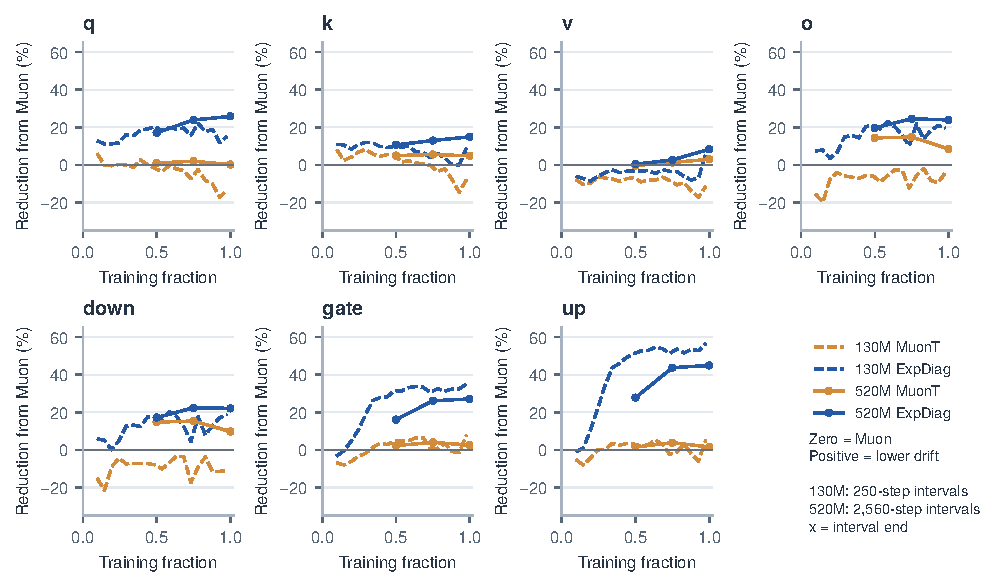
\includegraphics[width=\textwidth]{fig10_drift_by_role.pdf}
 \caption{\textbf{Fixed-data output-subspace drift reduction at each saved interval by projection role.} Curves show \mname{MuonT} and \mname{WT-MLP-Lag} relative to \mname{Muon} at the same model size and interval, averaging 32 layers and two probe sets before taking ratios (positive values denote lower drift than \mname{Muon}). Dashed curves show 130M (250-step intervals) and solid curves show 520M (2,560-step intervals, shared $\eta=0.016$) plotted against interval end as a fraction of total training steps (\Cref{tab:output_drift}).}
 \label{fig:output_drift_roles}
\end{figure}

\paragraph{Uninterrupted 130M training-EMA check.}
Separately, we compare saved dense output training EMAs ($\beta=0.938$) at every 250-step checkpoint from 250 to 5,000 between \mname{WT-MLP-Lag} and a passive \mname{MuonT} control (which records output EMAs on seed 0 at $\eta=0.02263$ while applying identity output factors; \mname{Muon} saved no output EMAs, and \mname{WT} stores only diagonals on \texttt{gate,up}, leaving the five $\dm$-wide roles \texttt{q,k,v,o,down} over 19 equal intervals plus the separate $5{,}000\text{--}5{,}120$ tail). Averaged over layers and intervals, \mname{WT} lowers top-16 EMA drift by $16.3\%,12.0\%,11.4\%,7.8\%$, and $28.0\%$ on \texttt{q,k,v,o,down}, winning $17,15,19,11$, and $17$ of $19$ intervals (\texttt{o} has higher early drift and lower late drift; because the passive control uses per-matrix updates while \mname{WT} uses batched lagged updates, this EMA check is descriptive rather than strictly causal).

\paragraph{Subspace rank, boundary-gap filtering, and finite-probe scope.}
Repeating fixed-data comparisons against \mname{Muon} at $k\in\{8,16,32,64\}$ preserves positive average reductions across all seven roles in each probe set separately at matched $\eta=0.016$—both at 520M and on all three fresh 130M seeds—whereas on the mixed-rate 130M seed-0 curve \texttt{q, k, o, down, gate, up} remain positive and \texttt{v} remains higher at every tested $k$ in each probe set. On training EMAs, \texttt{q, v, down} remain positive across all $k$, whereas \texttt{o} reverses at $k=32,64$ and \texttt{k} at $k=64$. Restricting $k=16$ comparisons to layer--interval--probe observations with relative boundary gap $(\lambda_{16}-\lambda_{17})/\lambda_{16}\ge1\%$ at both endpoints in both compared methods (retaining 47--93\% of pooled observations across roles at 130M and 52--95\% at 520M, weighted equally) preserves all sign patterns in both fixed-data and EMA audits. FP64 eigensolve residuals $\|BV-V\Lambda\|_F/\|B\|_F$ are at most $2.6\times10^{-15}$ prior to FP32 storage. Finally, finite 4,576-row probe sets do not recover exact population subspaces (for instance, at 520M the same-checkpoint top-16 distance between the two disjoint probe sets averages $0.941$ on \mname{Muon}'s \texttt{gate}, $0.924$ on \mname{MuonT}'s, and $0.750$ on \mname{WT}'s; we do not subtract this cross-set distance from temporal drift).

\FloatBarrier
\section{Learning-rate selection and complete losses}
\label{app:appendix_lr}

The short-schedule sweep uses 320 updates with a full decay schedule compressed into that 0.17B-token horizon (\Cref{tab:lr_cliff}). Whereas 320-step sweeps favor $\eta\in[0.064,0.0905]$, full 5,120-step curves achieve a strict interior minimum at $\eta^*=0.0160$ across all four core methods and degrade by $0.04\text{--}0.09$ nats when run at their 320-step argmax rates (\Cref{tab:controls,tab:lr_cliff}). Similarly, at 130M and 80 TPP, scaling from the hotter $\eta=0.02263$ rate ($\eta=0.01493$) yields $+0.00358$ nats Paloma macro difference from \mname{MuonT} versus $-0.00566$ nats at the matched horizon-scaled rate $\eta=0.01056$ (\Cref{tab:absolute_results}), underscoring how learning-rate mismatch can flip apparent second-side conclusions. Complete absolute losses and replicates at both $\eta=0.01600$ and $\eta=0.02263$—across fresh 130M seeds 1--3 and all four 520M methods, where every 520M optimizer achieves lower held-out and C4 loss at $0.01600$—appear in \Cref{tab:absolute_results,tab:seeds}.

\begin{table}[tbp]\centering\footnotesize
\setlength{\tabcolsep}{5.2pt}
\caption{\textbf{Short-schedule (320-step) versus full-budget (5,120-step) matrix learning-rate sweeps at 130M (seed 0).} Entries are final held-out losses $\Lsel$ in nats; bold marks each row's minimum within that horizon. All four core full-budget curves achieve an interior minimum at $0.0160$, whereas the compressed 320-step schedule shifts apparent optima $4\text{--}6\times$ higher.}\label{tab:lr_cliff}
\begin{tabularx}{\textwidth}{@{}>{\raggedright\arraybackslash}Xrrrrrrrr@{}}
\toprule
Method & 0.0113 & 0.0160 & 0.0226 & 0.0320 & 0.0453 & 0.0640 & 0.0905 & 0.1280 \\
\midrule
\addlinespace[2pt]\multicolumn{9}{@{}l}{\textit{Short-schedule proxy sweep: 320 steps (0.17B tokens, seed 0)}}\\
MuonT & --- & 4.5661 & 4.4221 & 4.3347 & 4.2720 & \textbf{4.2510} & 4.2533 & 4.3021 \\
Muon2-Diag & --- & 4.5787 & 4.4312 & 4.3326 & 4.2577 & 4.2339 & \textbf{4.2314} & 4.2693 \\
Abl-OuterDiag & --- & 4.5854 & 4.4417 & 4.3337 & 4.2702 & 4.2442 & \textbf{4.2367} & 4.2798 \\
Abl-OuterDiag-F & --- & 4.5887 & 4.4412 & 4.3346 & 4.2748 & \textbf{4.2411} & 4.2436 & 4.2878 \\
\addlinespace[5pt]\multicolumn{9}{@{}l}{\textit{Full-budget verification: 5,120 steps (2.68B tokens, seed 0)}}\\
Muon & 3.2496 & \textbf{3.2461} & 3.2524 & 3.2667 & --- & --- & --- & --- \\
MuonT & 3.2404 & \textbf{3.2342} & 3.2354 & 3.2398 & --- & 3.2775 & --- & --- \\
Muon2-Diag & 3.2383 & \textbf{3.2318} & 3.2333 & 3.2403 & --- & --- & 3.3200 & --- \\
Abl-OuterDiag-F & --- & --- & \textbf{3.2318} & --- & --- & 3.2752 & --- & --- \\
\rowcolor{rowtint}[0pt][0pt]\textbf{Muon2-ExpDiag} & 3.2363 & \textbf{3.2303} & 3.2311 & 3.2356 & --- & --- & --- & --- \\
\bottomrule\end{tabularx}
\end{table}

\begin{table}[tbp]\centering\scriptsize
\setlength{\tabcolsep}{8.5pt}
\caption{\textbf{Complete absolute losses and learning rates across all confirmatory regimes.} All losses are cross-entropy in nats; Late-11 Held-out averages the 11 second-half evaluation checkpoints. Hotter-LR rows ($\eta=0.02263$ at 130M and 520M 20 TPP; $\eta=0.01493$ at 130M 80 TPP) document the two-rate checks and learning-rate sensitivity discussed in \Cref{sec:phase2,sec:phase3,sec:phase4}.}\label{tab:absolute_results}
\begin{tabularx}{\textwidth}{@{}>{\raggedright\arraybackslash}Xrrrrr@{}}
\toprule
Method & Matrix $\eta$ & Final Held-out & Late-11 Held-out & Final C4 & Paloma Macro \\
\midrule
\addlinespace[2pt]\multicolumn{6}{@{}l}{\textit{130M seed-0 controls: 20 TPP, 2.68B tokens (complete learning-rate bracket)}}\\
Muon & 0.01131 & 3.2496 & 3.3692 & 3.4661 & 3.4179 \\
MuonT & 0.01131 & 3.2404 & 3.3521 & 3.4589 & 3.4154 \\
Muon2-Diag & 0.01131 & 3.2383 & 3.3500 & 3.4569 & 3.4115 \\
Muon2-ExpDiag & 0.01131 & 3.2363 & 3.3476 & 3.4548 & 3.4088 \\
Muon & 0.01600 & 3.2461 & 3.3824 & 3.4618 & --- \\
MuonT & 0.01600 & 3.2342 & 3.3591 & 3.4511 & 3.4041 \\
Muon2-Diag & 0.01600 & 3.2318 & 3.3555 & 3.4475 & 3.4048 \\
Muon2-ExpDiag & 0.01600 & 3.2303 & 3.3544 & 3.4472 & 3.3985 \\
Muon & 0.02263 & 3.2524 & 3.4064 & 3.4675 & --- \\
MuonT & 0.02263 & 3.2354 & 3.3763 & 3.4511 & 3.4021 \\
Null-Ctrl & 0.02263 & 3.2351 & 3.3755 & 3.4506 & --- \\
Muon2-Diag & 0.02263 & 3.2333 & 3.3724 & 3.4489 & --- \\
Muon2-ExpDiag & 0.02263 & 3.2311 & 3.3716 & 3.4491 & 3.4019 \\
Muon & 0.03200 & 3.2667 & 3.4426 & 3.4819 & 3.4313 \\
MuonT & 0.03200 & 3.2398 & 3.3970 & 3.4563 & --- \\
Muon2-Diag & 0.03200 & 3.2403 & 3.3981 & 3.4563 & --- \\
Muon2-ExpDiag & 0.03200 & 3.2356 & 3.3947 & 3.4533 & --- \\
\addlinespace[4pt]\multicolumn{6}{@{}l}{\textit{130M confirmation: 20 TPP, 2.68B tokens (mean of fresh seeds 1--3; matched $\eta^*$ \& hotter LR)}}\\
Muon & 0.01600 & 3.2035 & 3.3375 & 3.4640 & 3.4164 \\
MuonT & 0.01600 & 3.1916 & 3.3143 & 3.4523 & 3.4049 \\
Muon2-Diag & 0.01600 & 3.1919 & 3.3146 & 3.4514 & 3.4036 \\
\rowcolor{rowtint}[0pt][0pt]Muon2-ExpDiag & 0.01600 & 3.1881 & 3.3107 & 3.4484 & 3.4005 \\
Muon2-Diag (hotter LR) & 0.02263 & 3.1911 & 3.3282 & 3.4493 & 3.4040 \\
Muon2-ExpDiag (hotter LR) & 0.02263 & 3.1883 & 3.3265 & 3.4488 & 3.4009 \\
\addlinespace[4pt]\multicolumn{6}{@{}l}{\textit{130M longer training: 80 TPP, 10.74B tokens, seed 0 (matched \& hotter rates)}}\\
Muon & 0.01056 & 3.0778 & 3.2236 & 3.2989 & 3.2479 \\
MuonT & 0.01056 & 3.0675 & 3.2013 & 3.2886 & 3.2368 \\
Muon2-Diag & 0.01056 & 3.0656 & 3.1997 & 3.2861 & 3.2342 \\
\rowcolor{rowtint}[0pt][0pt]Muon2-ExpDiag & 0.01056 & 3.0636 & 3.1967 & 3.2848 & 3.2312 \\
Muon2-ExpDiag (hotter LR) & 0.01493 & 3.0696 & 3.2203 & 3.2900 & 3.2404 \\
\addlinespace[4pt]\multicolumn{6}{@{}l}{\textit{520M width transfer: 20 TPP, 10.74B tokens, seed 0 (matched $\eta^*$ \& hotter rates)}}\\
Muon & 0.01600 & 2.8528 & 2.9858 & 3.0769 & 3.0291 \\
MuonT & 0.01600 & 2.8438 & 2.9658 & 3.0696 & 3.0256 \\
Muon2-Diag & 0.01600 & 2.8433 & 2.9638 & 3.0674 & 3.0262 \\
\rowcolor{rowtint}[0pt][0pt]Muon2-ExpDiag & 0.01600 & 2.8392 & 2.9611 & 3.0653 & 3.0179 \\
Muon (hotter LR) & 0.02263 & 2.8639 & 3.0153 & 3.0860 & 3.0379 \\
MuonT (hotter LR) & 0.02263 & 2.8463 & 2.9839 & 3.0704 & 3.0256 \\
Muon2-Diag (hotter LR) & 0.02263 & 2.8469 & 2.9845 & 3.0708 & 3.0261 \\
Muon2-ExpDiag (hotter LR) & 0.02263 & 2.8435 & 2.9809 & 3.0682 & 3.0202 \\
\bottomrule\end{tabularx}
\end{table}

\begin{table}[tbp]\centering\footnotesize
\setlength{\tabcolsep}{7.5pt}
\caption{\textbf{Individual fresh-seed replication at 130M (20 TPP, 2.68B tokens).} Subheaders report each seed's absolute Muon losses ($\eta^*=0.01600$); rows report paired differences from same-seed Muon in millinats (negative favors the row method; Late-11 is omitted for $\eta=0.02263$ rows because intermediate decay schedules differ). Muon2-ExpDiag improves over both Muon and MuonT on every seed across all evaluation suites at both learning rates.}\label{tab:seeds}
\begin{tabularx}{\textwidth}{@{}>{\raggedright\arraybackslash}Xrrrrr@{}}
\toprule
Method & Matrix $\eta$ & $\Delta$ Held-out & Late-11 $\Delta$ & $\Delta$ C4 & $\Delta$ Paloma \\
\midrule
\addlinespace[2pt]\multicolumn{6}{@{}l}{\textit{Seed 1: Muon reference ($\Lsel=3.2003$, Late-11 $=3.3362$, $\Lc=3.4655$, $\Lpal=3.4162$ nats)}}\\
MuonT & 0.01600 & $-12.44$ & $-24.87$ & $-12.66$ & $-11.64$ \\
Muon2-Diag & 0.01600 & $-11.83$ & $-24.08$ & $-13.10$ & $-11.90$ \\
\rowcolor{rowtint}[0pt][0pt]\textbf{Muon2-ExpDiag} & 0.01600 & $\mathbf{-14.02}$ & $\mathbf{-26.50}$ & $\mathbf{-16.18}$ & $\mathbf{-15.69}$ \\
Muon2-Diag (hotter LR) & 0.02263 & $-13.46$ & --- & $-16.73$ & $-14.26$ \\
Muon2-ExpDiag (hotter LR) & 0.02263 & $-15.31$ & --- & $-17.01$ & $-15.99$ \\
\addlinespace[4pt]\multicolumn{6}{@{}l}{\textit{Seed 2: Muon reference ($\Lsel=3.1764$, Late-11 $=3.3089$, $\Lc=3.4639$, $\Lpal=3.4182$ nats)}}\\
MuonT & 0.01600 & $-12.97$ & $-23.99$ & $-11.98$ & $-15.59$ \\
Muon2-Diag & 0.01600 & $-12.58$ & $-23.61$ & $-13.55$ & $-14.99$ \\
\rowcolor{rowtint}[0pt][0pt]\textbf{Muon2-ExpDiag} & 0.01600 & $\mathbf{-17.93}$ & $\mathbf{-29.22}$ & $\mathbf{-17.11}$ & $\mathbf{-17.68}$ \\
Muon2-Diag (hotter LR) & 0.02263 & $-12.99$ & --- & $-14.58$ & $-10.86$ \\
Muon2-ExpDiag (hotter LR) & 0.02263 & $-15.21$ & --- & $-15.43$ & $-16.75$ \\
\addlinespace[4pt]\multicolumn{6}{@{}l}{\textit{Seed 3: Muon reference ($\Lsel=3.2339$, Late-11 $=3.3675$, $\Lc=3.4627$, $\Lpal=3.4148$ nats)}}\\
MuonT & 0.01600 & $-10.33$ & $-20.92$ & $-10.73$ & $-7.25$ \\
Muon2-Diag & 0.01600 & $-10.44$ & $-21.04$ & $-11.25$ & $-11.48$ \\
\rowcolor{rowtint}[0pt][0pt]\textbf{Muon2-ExpDiag} & 0.01600 & $\mathbf{-14.27}$ & $\mathbf{-24.63}$ & $\mathbf{-13.63}$ & $\mathbf{-14.35}$ \\
Muon2-Diag (hotter LR) & 0.02263 & $-10.91$ & --- & $-12.77$ & $-12.02$ \\
Muon2-ExpDiag (hotter LR) & 0.02263 & $-15.32$ & --- & $-13.42$ & $-13.78$ \\
\bottomrule\end{tabularx}
\end{table}


\FloatBarrier
\section{Placement ablations}
\label{app:ablations}

\Cref{tab:ablations_full} reports all 19 exploratory factor-placement, exponent, and scheduling arms at 130M alongside each arm's same-wave \mname{MuonT} reference. Because earlier waves (W0--W3, W10) precede the unified fast-lag confirmation runner, cross-wave comparisons are exploratory; the matched-path controls and multi-seed confirmation runs in \Cref{sec:scaling,sec:falsification} provide the primary test of \mname{WT-MLP-Lag}.

\begin{table}[tbp]\centering\footnotesize
\setlength{\tabcolsep}{3.1pt}
\caption{\textbf{Complete 19-arm placement and operator ledger at 130M (seed 0, 2.68B tokens).} Cohort identifies the implementation wave providing each arm's paired MuonT reference (W0--W4, W10, or FastLag); loss columns report cohort-adjusted differences (millinats) relative to Muon ($\text{arm}-\text{cohort MuonT}$ shifted by W0 MuonT minus Muon, which equals raw difference from Muon on W0--W4; Late averages 11 second-half checkpoints; Train averages the final 537M tokens). Step $\Delta t$ is median overhead relative to Muon in the unified 8-GPU benchmark. Because earlier waves precede the unified confirmation runner, cross-wave differences are exploratory.}\label{tab:ablations_full}
\begin{tabularx}{\textwidth}{@{}>{\raggedright\arraybackslash}Xlllrrrrr@{}}
\toprule
& & ($\dm/\dff$) & ($\dm/\dff$) & \multicolumn{4}{c}{$\Delta$ vs.\ Muon (mnats, $\downarrow$)} & \\
\cmidrule(lr){5-8}
Method & Cohort & Inputs & Outputs & Final & Late & Late C4 & Train & Step $\Delta t$ \\
\midrule
\addlinespace[2pt]\multicolumn{9}{@{}l}{\textit{Reference baselines and execution-path control}}\\
Muon & W0 & $I$ / $I$ & $I$ / $I$ & $+0.00$ & $+0.00$ & $+0.00$ & $+0.00$ & $+0.0\%$ \\
MuonT & W0 & Dense / Dense & $I$ / $I$ & $-9.48$ & $-5.50$ & $-5.34$ & $-6.16$ & $+1.5\%$ \\
Null-Ctrl & W3 & Dense / Dense & $I$ / $I$ (solved) & $-10.82$ & $-6.15$ & $-7.39$ & $-6.85$ & $+13.9\%$ \\
Null-Dense & W1 & Dense / Dense & $I$ / $I$ (solved) & $-10.65$ & $-6.79$ & $-7.64$ & $-7.52$ & $+27.5\%$ \\
Null-Diag & W10 & Dense / Dense & $I$ / $I$ (solved) & $-10.89$ & $-7.51$ & $-6.57$ & $-7.30$ & $+2.9\%$ \\
\addlinespace[4pt]\multicolumn{9}{@{}l}{\textit{Replacing or weakening input whitening}}\\
Abl-BothDiag & W1 & Diag / Diag & Diag / Diag & $-2.15$ & $+12.51$ & $+12.34$ & $+7.21$ & $+1.1\%$ \\
Abl-OutOnly & W1 & $I$ / $I$ & Dense / Dense & $-6.23$ & $+3.20$ & $+5.55$ & $+1.71$ & $+31.7\%$ \\
Abl-DownSwap & W0 & Dense / $I$ & $I$ (\texttt{down} Dense) & $-8.42$ & $-2.99$ & $-1.74$ & $-2.98$ & $+1.8\%$ \\
Abl-SymDiag (sync) & FastLag & Dense / Diag & Dense / Diag & $-12.48$ & $-8.02$ & $-7.37$ & $-7.42$ & $+10.9\%$ \\
Abl-SymDiag & FastLag & Dense / Diag & Dense / Diag & $-11.94$ & $-6.63$ & $-6.95$ & $-7.64$ & $+4.8\%$ \\
\addlinespace[4pt]\multicolumn{9}{@{}l}{\textit{Output projection role and inner/outer exponent placement}}\\
Abl-DownOnly & W0 & Dense / Dense & $\hat L_{\rm down}$ only & $-10.76$ & $-6.87$ & $-6.13$ & $-7.32$ & $+3.6\%$ \\
Abl-OuterDiag & W10 & Dense / Dense & $\hat L$ Diag / $\hat L$ Diag & $-11.27$ & $-7.96$ & $-7.94$ & $-7.54$ & $+3.0\%$ \\
Abl-NoExp & W2 & Dense / Dense & Dense / $I$ & $-12.59$ & $-8.57$ & $-7.97$ & $-8.29$ & $+13.7\%$ \\
Abl-OuterDense & W2 & Dense / Dense & $\hat L$ Dense ($L=I$) & $-13.67$ & $-9.48$ & $-10.12$ & $-10.04$ & $+28.2\%$ \\
Muon2-Diag & W2 & Dense / Dense & Diag / Diag & $-13.62$ & $-10.01$ & $-8.95$ & $-9.85$ & $+3.7\%$ \\
\addlinespace[4pt]\multicolumn{9}{@{}l}{\textit{Dense two-sided ceiling versus expansion-diagonal outputs and one-step lag}}\\
Muon2-Dense & W1 & Dense / Dense & Dense / Dense & $-15.63$ & $-11.29$ & $-11.72$ & $-11.14$ & $+23.3\%$ \\
Muon2-Dense (lag) & W3 & Dense / Dense & Dense / Dense & $-15.69$ & $-11.40$ & $-11.21$ & $-11.89$ & $+18.2\%$ \\
Muon2-ExpDiag (sync) & W2 & Dense / Dense & Dense / Diag & $\mathbf{-16.37}$ & $\mathbf{-12.09}$ & $-11.42$ & $-11.23$ & $+12.9\%$ \\
\rowcolor{rowtint}[0pt][0pt]\textbf{Muon2-ExpDiag} & W4 & Dense / Dense & Dense / Diag & $\mathbf{-16.04}$ & $\mathbf{-11.19}$ & $\mathbf{-10.33}$ & $\mathbf{-11.11}$ & $+6.8\%$ \\
\bottomrule\end{tabularx}
\end{table}


\FloatBarrier
\section{Systems measurements and domain evaluation}
\label{app:appendix_systems}

The unified 130M timing benchmark (\Cref{tab:bench19}) initializes all 19 arms from identical step-2,500 weights with fresh optimizer/moment state on $8\times\text{A100}$, warms up for 36 steps, and records rank-0 real-data training step durations over steps 37--96 (including data loading and distributed gradient synchronization, excluding compilation, evaluation, and checkpoint I/O). One 60-step window per arm does not resolve sub-percent differences or per-rank maxima. The 520M records (\Cref{tab:bench520m}) report complete windows without outlier removal across both matched-checkpoint initialization (steps 37--96) and each method's own warmed step-5,120 optimizer state (steps 17--76) on $8\times$ and $32\times\text{A100}$ GPUs. Complete 16-domain Paloma scores appear in \Cref{tab:paloma_full}.

\begin{table}[tbp]\centering\footnotesize
\setlength{\tabcolsep}{9.5pt}
\caption{\textbf{Complete 19-arm 130M timing and memory benchmark on 8$\times$A100.} Sorted by median step duration over steps 37--96 (after 36 warmup steps) from identical step-2,500 weights and fresh optimizer/moment state. Both median and mean overheads ($\Delta$) are relative to Muon.}\label{tab:bench19}
\begin{tabularx}{\textwidth}{@{}>{\raggedright\arraybackslash}Xrrrrr@{}}
\toprule
Method & Median (s) & Median $\Delta$ & Mean (s) & Mean $\Delta$ & Peak GiB \\
\midrule
Muon & 1.0810 & $+0.0\%$ & 1.0792 & $+0.0\%$ & 18.97 \\
Abl-BothDiag & 1.0926 & $+1.1\%$ & 1.0911 & $+1.1\%$ & 19.55 \\
MuonT & 1.0967 & $+1.5\%$ & 1.0971 & $+1.7\%$ & 20.54 \\
Abl-DownSwap & 1.1005 & $+1.8\%$ & 1.0976 & $+1.7\%$ & 19.41 \\
Null-Diag & 1.1121 & $+2.9\%$ & 1.1121 & $+3.0\%$ & 20.55 \\
Abl-OuterDiag & 1.1131 & $+3.0\%$ & 1.1134 & $+3.2\%$ & 20.55 \\
Abl-DownOnly & 1.1202 & $+3.6\%$ & 1.1283 & $+4.5\%$ & 20.76 \\
Muon2-Diag & 1.1211 & $+3.7\%$ & 1.1196 & $+3.7\%$ & 20.55 \\
Abl-SymDiag & 1.1331 & $+4.8\%$ & 1.1751 & $+8.9\%$ & 20.82 \\
\rowcolor{rowtint}[0pt][0pt]\textbf{Muon2-ExpDiag} & 1.1548 & $+6.8\%$ & 1.1944 & $+10.7\%$ & 21.60 \\
Abl-SymDiag (sync) & 1.1986 & $+10.9\%$ & 1.2356 & $+14.5\%$ & 20.74 \\
Muon2-ExpDiag (sync) & 1.2208 & $+12.9\%$ & 1.2501 & $+15.8\%$ & 21.52 \\
Abl-NoExp & 1.2288 & $+13.7\%$ & 1.2517 & $+16.0\%$ & 21.52 \\
Null-Ctrl & 1.2313 & $+13.9\%$ & 1.2493 & $+15.8\%$ & 21.52 \\
Muon2-Dense (lag) & 1.2782 & $+18.2\%$ & 1.4585 & $+35.1\%$ & 24.78 \\
Muon2-Dense & 1.3333 & $+23.3\%$ & 1.4595 & $+35.2\%$ & 24.21 \\
Null-Dense & 1.3785 & $+27.5\%$ & 1.4638 & $+35.6\%$ & 24.21 \\
Abl-OuterDense & 1.3861 & $+28.2\%$ & 1.5004 & $+39.0\%$ & 24.21 \\
Abl-OutOnly & 1.4232 & $+31.7\%$ & 1.4579 & $+35.1\%$ & 22.21 \\
\bottomrule\end{tabularx}
\end{table}

\begin{table}[tbp]\centering\footnotesize
\setlength{\tabcolsep}{9.5pt}
\caption{\textbf{Complete 520M timing and memory records across 8 and 32 A100 GPUs (1.0M batch, chunked buffers).} All rows report the complete recorded measurement window without outlier removal; own optimizer states restore each arm's converged step-5,120 moments and eigenbases. Overheads ($\Delta$) are relative to within-group Muon.}\label{tab:bench520m}
\begin{tabularx}{\textwidth}{@{}>{\raggedright\arraybackslash}Xrrrrr@{}}
\toprule
Method & Median (s) & Median $\Delta$ & Mean (s) & Mean $\Delta$ & Peak GiB \\
\midrule
\addlinespace[2pt]\multicolumn{6}{@{}l}{\textit{8 GPUs, matched checkpoint, steps 37--96}}\\
Muon & 4.6419 & $+0.0\%$ & 4.6456 & $+0.0\%$ & 26.46 \\
MuonT & 4.8943 & $+5.4\%$ & 4.9010 & $+5.5\%$ & 29.05 \\
Muon2-Diag & 4.9863 & $+7.4\%$ & 4.9902 & $+7.4\%$ & 29.06 \\
\rowcolor{rowtint}[0pt][0pt]\textbf{Muon2-ExpDiag} & 5.3219 & $+14.6\%$ & 5.3181 & $+14.5\%$ & 30.73 \\
\addlinespace[4pt]\multicolumn{6}{@{}l}{\textit{32 GPUs, matched checkpoint, steps 37--96}}\\
Muon & 1.3222 & $+0.0\%$ & 1.3241 & $+0.0\%$ & 26.46 \\
MuonT & 1.3851 & $+4.8\%$ & 1.3911 & $+5.1\%$ & 26.93 \\
Muon2-Diag & 1.4063 & $+6.4\%$ & 1.4119 & $+6.6\%$ & 26.94 \\
\rowcolor{rowtint}[0pt][0pt]\textbf{Muon2-ExpDiag} & 1.4305 & $+8.2\%$ & 1.5493 & $+17.0\%$ & 27.88 \\
\addlinespace[4pt]\multicolumn{6}{@{}l}{\textit{32 GPUs, own optimizer states, steps 17--76}}\\
Muon & 1.3124 & $+0.0\%$ & 1.3163 & $+0.0\%$ & 26.46 \\
MuonT & 1.3809 & $+5.2\%$ & 1.3853 & $+5.2\%$ & 26.93 \\
Muon2-Diag & 1.4203 & $+8.2\%$ & 1.4453 & $+9.8\%$ & 26.94 \\
\rowcolor{rowtint}[0pt][0pt]\textbf{Muon2-ExpDiag} & 1.4578 & $+11.1\%$ & 1.5388 & $+16.9\%$ & 27.88 \\
\addlinespace[4pt]\multicolumn{6}{@{}l}{\textit{8 GPUs, own optimizer states, steps 17--76}}\\
Muon & 4.6383 & $+0.0\%$ & 4.6396 & $+0.0\%$ & 26.46 \\
MuonT & 4.8779 & $+5.2\%$ & 4.8994 & $+5.6\%$ & 29.05 \\
Muon2-Diag & 5.0287 & $+8.4\%$ & 5.0533 & $+8.9\%$ & 29.07 \\
\rowcolor{rowtint}[0pt][0pt]\textbf{Muon2-ExpDiag} & 5.6081 & $+20.9\%$ & 5.6098 & $+20.9\%$ & 30.74 \\
\bottomrule\end{tabularx}
\end{table}

\begin{table}[tbp]\centering\small
\setlength{\tabcolsep}{7.0pt}
\caption{\textbf{Per-domain Paloma loss differences from MuonT across all 16 domains.} Entries are millinats ($\text{Method}-\text{MuonT}$; negative favors the method, bold marks the stronger output approximation within each regime). The 130M 20-TPP columns average paired differences across fresh seeds 1--3; 130M 80-TPP and 520M 20-TPP use single-seed matched-rate runs.}\label{tab:paloma_full}
\begin{tabularx}{\textwidth}{@{}>{\raggedright\arraybackslash}Xrrrrrr@{}}
\toprule
& \multicolumn{2}{c}{130M, 20 TPP (3 seeds)} & \multicolumn{2}{c}{130M, 80 TPP} & \multicolumn{2}{c}{520M, 20 TPP} \\
\cmidrule(lr){2-3}\cmidrule(lr){4-5}\cmidrule(lr){6-7}
Paloma domain & OD-All & WT-Lag & OD-All & WT-Lag & OD-All & WT-Lag \\
\midrule
C4-EN & $-0.85$ & $\mathbf{-3.86}$ & $-2.55$ & $\mathbf{-3.80}$ & $-2.14$ & $\mathbf{-4.27}$ \\
C4 domains & $-0.98$ & $\mathbf{-3.78}$ & $-1.85$ & $\mathbf{-4.07}$ & $-0.98$ & $\mathbf{-2.92}$ \\
mC4 & $+0.29$ & $\mathbf{-3.73}$ & $-1.08$ & $\mathbf{-2.66}$ & $-2.76$ & $\mathbf{-6.36}$ \\
Dolma & $-1.12$ & $\mathbf{-4.13}$ & $-2.23$ & $\mathbf{-4.35}$ & $-1.95$ & $\mathbf{-3.58}$ \\
RefinedWeb & $-1.10$ & $\mathbf{-3.96}$ & $-3.43$ & $\mathbf{-5.00}$ & $-1.99$ & $\mathbf{-3.63}$ \\
RedPajama & $-0.73$ & $\mathbf{-2.81}$ & $-3.63$ & $\mathbf{-4.11}$ & $-1.75$ & $\mathbf{-8.12}$ \\
Wikipedia & $-0.75$ & $\mathbf{-3.88}$ & $-2.51$ & $\mathbf{-4.80}$ & $-0.00$ & $\mathbf{-2.36}$ \\
S2ORC & $-0.51$ & $\mathbf{-4.35}$ & $-3.11$ & $\mathbf{-4.78}$ & $-0.67$ & $\mathbf{-3.93}$ \\
Programming & $+0.51$ & $\mathbf{-4.29}$ & $-0.77$ & $\mathbf{-0.91}$ & $-2.11$ & $\mathbf{-5.39}$ \\
WikiText-103 & $\mathbf{+2.05}$ & $+2.84$ & $-6.14$ & $\mathbf{-11.00}$ & $+4.43$ & $\mathbf{-2.16}$ \\
Penn Treebank & $\mathbf{-9.42}$ & $-1.52$ & $-15.72$ & $\mathbf{-19.42}$ & $-0.15$ & $\mathbf{-7.17}$ \\
Subreddits & $+0.62$ & $\mathbf{-1.85}$ & $\mathbf{-3.34}$ & $-3.03$ & $-2.32$ & $\mathbf{-3.84}$ \\
TwitterAAE & $-6.94$ & $\mathbf{-19.72}$ & $+18.06$ & $\mathbf{-2.21}$ & $+8.74$ & $\mathbf{-59.67}$ \\
Manosphere & $-1.50$ & $\mathbf{-7.05}$ & $-0.57$ & $\mathbf{-1.46}$ & $-2.22$ & $\mathbf{-5.87}$ \\
4chan & $+2.33$ & $\mathbf{-3.40}$ & $-7.74$ & $\mathbf{-9.18}$ & $+3.44$ & $\mathbf{-2.78}$ \\
Gab & $-2.62$ & $\mathbf{-5.16}$ & $-4.86$ & $\mathbf{-9.87}$ & $+13.00$ & $\mathbf{-0.04}$ \\
\midrule
\rowcolor{rowtint}[0pt][0pt]\textbf{16-domain macro mean} & $-1.30$ & $\mathbf{-4.41}$ & $-2.59$ & $\mathbf{-5.66}$ & $+0.66$ & $\mathbf{-7.63}$ \\
\textbf{Domains won vs.\ MuonT} & 11/16 & \textbf{15/16} & 15/16 & \textbf{16/16} & 12/16 & \textbf{16/16} \\
\bottomrule\end{tabularx}
\end{table}

